\documentclass{article}
\usepackage[utf8]{inputenc}
\date{April 22, 2021}
\usepackage[margin=1in]{geometry}
\setlength{\parindent}{0pt}
\usepackage{fancyhdr}
\usepackage{amsfonts}
\pagestyle{fancy}
\cfoot{\thepage}
\lhead{Andi Tse}
\chead{Essential Factoring Skills}
\rhead{
\includegraphics[width=0.7cm]{angold.png}}
\usepackage{mathtools}
\usepackage{amsmath}
\usepackage[LGR,T1]{fontenc}
\usepackage[utf8]{inputenc}
\usepackage{lmodern}
\usepackage{microtype}
\usepackage{upgreek}
\usepackage[misc]{ifsym}
\usepackage{amsmath,amsthm,amssymb}
\usepackage{pgfplots}
	\usetikzlibrary{
		calc,
		patterns,
		positioning
	}
	\pgfplotsset{
		compat=1.16,
		samples=200,
		clip=false,
		my axis style/.style={
			axis x line=middle,
			axis y line=middle,
			legend pos=outer north east,
			axis line style={
				->,
			},
			legend style={
				font=\footnotesize
			},
			label style={
				font=\footnotesize
			},
			tick label style={
				font=\footnotesize
			},
			xlabel style={
				at={
					(ticklabel* cs:1)
				},
				anchor=west,
				font=\footnotesize,
			},
			ylabel style={
				at={
					(ticklabel* cs:1)
				},
				anchor=west,
				font=\footnotesize,
			},
			xlabel=$x$,
			ylabel=$y$
		},
	}
	\tikzset{
		>=stealth
	}

\usepackage{float}
\usepackage{caption}
	\captionsetup{
		format=plain,
		labelfont=bf,
		font=small,
		justification=centering
	}
\usepackage{verbatim}
\usepackage{ulem}
\usepackage{amsfonts}
\usepackage{amssymb}
\usepackage{float}
\usepackage{caption}
	\captionsetup{
		format=plain,
		labelfont=bf,
		font=small,
		justification=centering
	}
\title{Essential Factor Skills}
\author{Andi Tse}
\renewcommand{\familydefault}{\sfdefault}
\usepackage{lmodern}
\usepackage{scalerel}
\setcounter{MaxMatrixCols}{20}

\newcommand{\longdiv}{\smash{\mkern-0.43mu\vstretch{1.31}{\hstretch{.7}{)}}\mkern-5.2mu\vstretch{1.31}{\hstretch{.7}{)}}}}

\usepackage[cm]{sfmath}
\usepackage{hyperref}
\usepackage{mathptmx}
\setlength{\parskip}{1em}

\usepackage{tcolorbox}
\usepackage{tikz}
\hypersetup{
    colorlinks,
    citecolor=black,
    filecolor=black,
    linkcolor=black,
}
\renewcommand{\abstractname}{}


\begin{document}
\maketitle
\tableofcontents\bigskip\bigskip\bigskip\bigskip\bigskip\bigskip


\section{Admire the Beauty of Mathematics}
Before we start, let us take a minute to praise the beauty of Mathematics:

\begin{figure}[h]
    \centering
    \resizebox{\columnwidth}{!}{%
        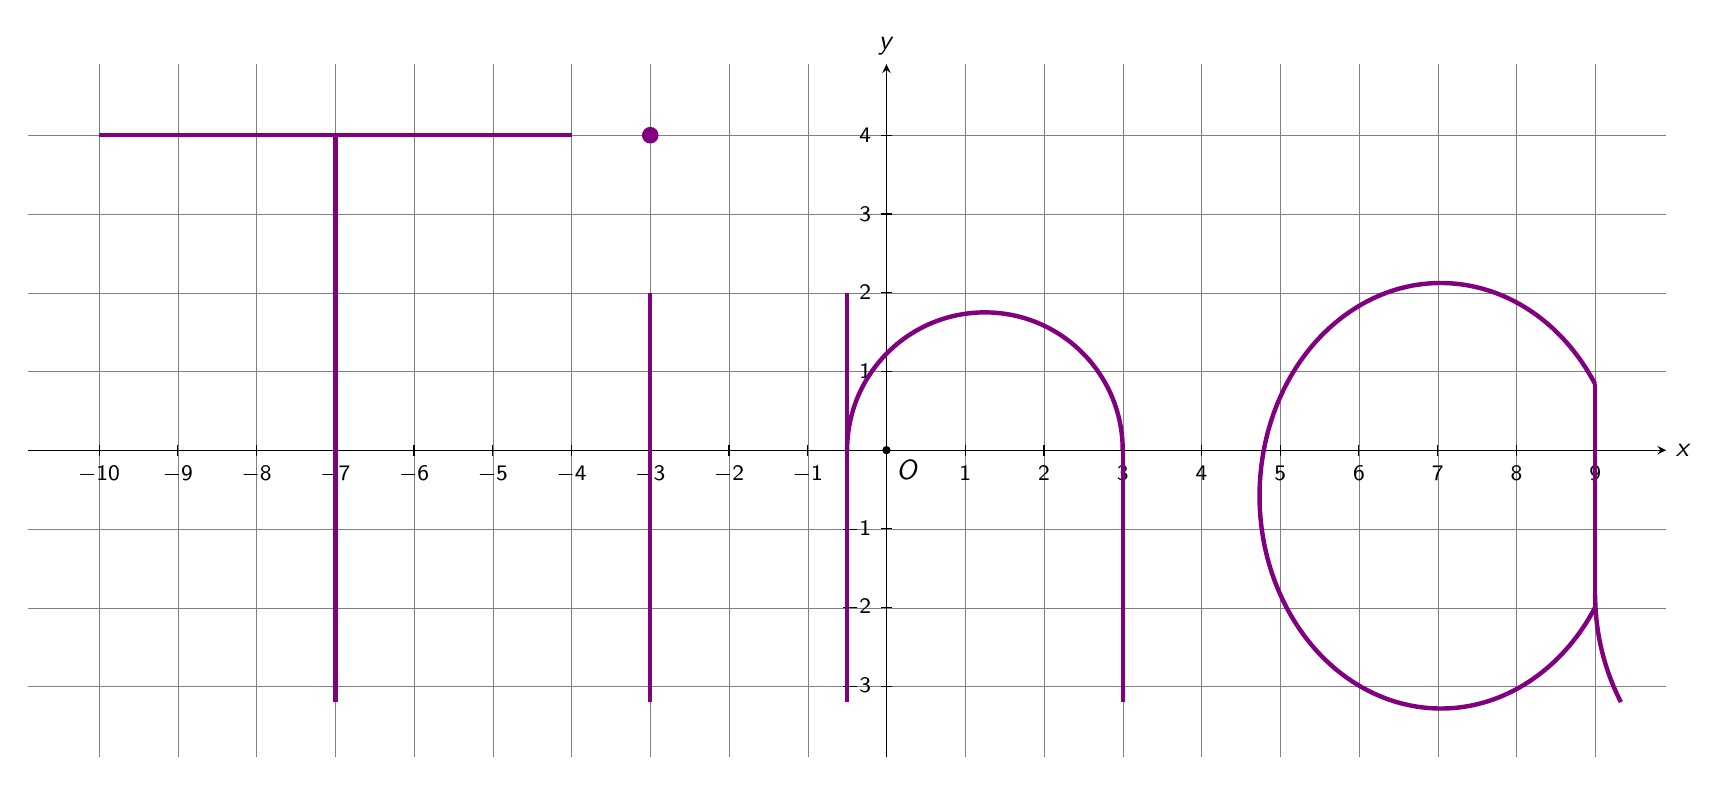
\begin{tikzpicture}
            \draw[xstep=1, ystep=1, gray, ultra thin] (-10.9,-3.9) grid (9.9,4.9);
            \draw[->] (-10.9, 0) -- (9.9, 0) node[right] [black] {$x$};
            \draw[->] (0, -3.9) -- (0, 4.9) node[above] [black] {$y$};
            \foreach \x in {-10,...,-1,1,2,...,9}
            \draw[shift={(\x,0)}] (0pt,2pt) -- (0pt,-2pt) node[below] {\footnotesize $\x$};
            \foreach \y in {-3,...,-1,1,2,...,4}
            \draw[shift={(0,\y)}] (2pt,0pt) -- (-2pt,0pt) node[left] {\footnotesize $\y$};
        	\fill[black] (0, 0) circle (1.5pt) node[below right] {$O$};

            
            \draw (-10, 4) -- (-4, 4) [violet] [ultra thick];
            \draw (-7, -3.2) -- (-7, 4) [violet] [ultra thick];
        	\fill[violet] (-3, 4) circle (3pt);
            \draw (-3, -3.2) -- (-3, 2) [violet] [ultra thick];
            \draw (-0.5, -3.2) -- (-0.5, 2) [violet] [ultra thick];
            \draw (3, 0) arc (0:180:1.75) [violet] [ultra thick];
            \draw (3, -3.2) -- (3, 0) [violet] [ultra thick];
            
            \draw (9,0.8381203375) arc(31.6314652982:328.368534702:2.30217288664 and 2.70185121722) [violet] [ultra thick];
            \draw (9, -2) -- (9, 0.83812) [violet] [ultra thick];
            \draw (9, -1.8381203375) arc (180: 207: 3) [violet] [ultra thick];

        \end{tikzpicture}
    }
\end{figure}
\pagebreak


\section{Introduction}
\textbf{Factoring} is arguably the most important skill in Algebra. Though it can involve all sorts of properties of different functions, the idea of factoring shares. In this handout, I will be using $x$ as the variable. Note that this can be changed to $\sin x,\  P(x),\ e^x$ etc. \medskip \\

\section{Distribute Law}
\textbf{Law of Distribution} is the formula $a(b+c)=ab+ac$. Notice that this formula is expanding the expression. When we reverse the equation, it becomes factoring! \emph{Factoring is the inverse process of expanding}.\medskip\\

\subsection{Example}
\begin{tcolorbox}
factor $x^2+3x$
\end{tcolorbox}

\subsubsection{Solution}
Notice that the \emph{Greatest Common Factor} of the two terms is $x$, so we extract the $x$. The answer is $x(x+3)$
\bigskip \bigskip

\subsection{Practices}
\begin{enumerate}
    \item Factor $7x-14$
    \item Factor $3x^2+6x$
    \item Factor $2x\left(x+1\right)+6x$
    \item Challenge Problem (credit, Jeffrey) $xy+x+y+1$
\end{enumerate}
\pagebreak


\section{Criss Cross Factoring}
LOL. I was laughing at how I did not know the name of this technique until working on this handout.

\includegraphics[width=0.5cm]{ango.png}\\\\
\textbf{Criss Cross Factoring} is especially useful when factoring quadratics. Because many of you may have already learned this. Allow me to explain why does it work ;-;
\subsection{Proof}
Remember that factoring is the inverse of expanding. Let's expand the polynomial $(ax+b)(cx+d)$

\begin{align*}
    &(ax+b)(cx+d)\\
    =\ &ax(cx+d)+b(cx+d)\\
    =\ &acx^2+adx+bcx+bd\\
    =\ &acx^2+(ad+bc)x+bd
\end{align*}
\medskip

This proves that an expression in the form of $(ax+b)(cx+d)$ can be expressed in $acx^2+(ad+bc)x+bd$. If we reverse this process, it becomes factoring. The goal is to find two pairs of factors in both the coefficient of $x^2$ and the constant term. Such that, as shown in the diagram below, the sum of the products of diagonals equals to the coeffiecient of $x$. \emph{Note that the order of $a,c$ matters}\medskip

% draw the criss cross diagram, this thing took me a whole day lol
\begin{center}
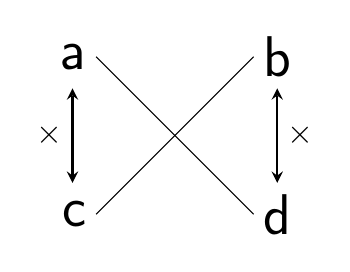
\begin{tikzpicture}
\draw (0, 0) -- (2, 2);
\draw (0, 2) -- (2, 0);
\draw (0, 0) node[left] {\huge c};
\draw (2, 0) node[right] {\huge d};
\draw (0, 2) node[left] {\huge a};
\draw (2, 2) node[right] {\huge b};
\draw[thick,<->] (-0.3,0.4) -- (-0.3, 1.6);
\draw[thick,<->] (2.3,0.4) -- (2.3, 1.6);
\draw (-0.3, 1) node[left] {\large $\times$};
\draw (2.3, 1) node[right] {\large $\times$};
\end{tikzpicture}
\end{center}


\subsection{Example}
\begin{tcolorbox}
Factor $x^2+3x+2$
\end{tcolorbox}
\medskip

\subsubsection{Solution}
The coefficient of $x^2$ is 1, whose combinations of factors has $(1, 1),(-1,-1)$ \\
The constant term is $2$, whose combinations of factors has $(1, 2),(2,1),(-1,-2),(-2,-1)$\\
After trying \sout{bashing} every combinations, we found out that the combination $(1,1),(1,2)$ works!

\begin{center}
\begin{tikzpicture}
\draw (0, 0) -- (2, 2);
\draw (0, 2) -- (2, 0);
\draw (0, 0) node[left] {\large 1};
\draw (2, -0.05) node[right] {\large 2};
\draw (0, 2) node[left] {\large 1};
\draw (2, 2) node[right] {\large 1};
\end{tikzpicture}
\end{center}
Now we have solved $a,b,c,d$, we can substitute the values into $(ax+b)(cx+d)$. The answer is $(x+1)(x+2)$


\subsection{Practices}
\begin{enumerate}
    \item Factor $x^2+5x+6$
    \item Factor $2x^2-x-1$
    \item Factor $x^2+\frac{7}{2}x+6$  (Hint: factor the $\frac{1}{2}$ first)
    \item Factor $2\sin^2x+3\sin x-2$
\end{enumerate}

% picture of angold follows
\pagebreak

\section{Special Binomial Products}
I personally think these three formulas are the formulas that I use the most in Algebra. I like to think of them as the "special cases" of \textit{criss cross factoring}. And I think they are really beautiful, look at their perfect symmetry! The maths below prove the expanding, so factoring is also proved. Let's go through the proofs for them. \sout{I tried to prove more interesting} ;-;\medskip

\subsection{Proof}
\subsubsection{Perfect Square Trinomials}
\begin{align*}
       &(a+b)^2       &       &(a-b)^2\\
    =\ &(a+b)(a+b)    &    =\ &\left(a+(-b)\right)^2\\
    =\ &a^2+ab+ab+b^2 &    =\ &a^2+2a(-b)+(-b)^2\\
    =\ &a^2+2ab+b^2   &    =\ &a^2-2ab+b^2
\end{align*}

\subsubsection{Difference of Squares}
\begin{align*}
       &(a+b)(a-b)\\
    =\ &a(a-b)+b(a-b)\\
    =\ &a^2-ab+ab-b^2\\
    =\ &a^2-b^2
\end{align*}
Proof without words:\\
\begin{center}
    \includegraphics[width = 15cm]{Diff of S no word.jpg}
\end{center}

\subsection{Example}
\begin{tcolorbox}
    Factor $4x^2+12x+9$
\end{tcolorbox}
\subsubsection{Solution}
We begin by notice that $4$ and $9$ are squares of $2$ and $3$ respectively, and $2\times 2\times 3 = 12$, which matches the coefficient of $x$. Therefore, the answer is $\left(2x+3\right)^2$


\subsection{Practices}
\begin{enumerate}
    \item Factor $9x^2+6x+1$
    \item Factor $4x^2+24x+144$
    \item Factor $x^4-1$
    \item Factor $2x^2+2\sqrt{6}x+3$
    \item Complete the square: $4x^2+6x+11$
\end{enumerate}
\parindent \emph{Complete the Square} is to convert a quadratic into the form $a(x+b)^2+c$, where $a,b,c$ are constants


\pagebreak
\section{Rational Root Theorem aka. Factor Theorem}
Now here is the big boi part lol. I find this theorem useful because it applies to any degree of polynomial. We begin by letting $Q(x)=(ax-b)P(x)+k\ \left(a,b\in \mathbb{Z},k\in \mathbb{R}\right)$. We will try to factor $Q(x)$.

\subsection{Proof}
\begin{center}
    Notice that when we substitute $x=\frac{b}{a}$ into $Q(x)$, $Q\left(\frac{b}{a}\right)=k$\\
    In order to factor $Q(x)$, we need to make $k=0$\\
    $\therefore Q(x)=Q\left(\frac{b}{a}\rigt)=0$\\
    What this means is that we need to find a value of $x,\ x=\frac{b}{a},$ that will make $Q(x)=0$\bigskip\bigskip
    
    Now let's see how do we find $\frac{b}{a}$.\\
    $Q(x)=(ax-b)P(x)$\\
    since $P(x)$ is a polynomial, we let $P(x)=gx^n+hx^{n-1}+\dots +j\ \left(g,h,j\in \mathbb{Z}\right)$ We don't care the part at the middle\\
    $\therefore Q(x)=agx^{n+1}+\dots -bj$\\
    \bigskip\bigskip
    
    Note that the above is expanding. In a problem that involves RRT, $Q(x)$ is often given. $a,b$ are the factors of the highest term and the constant term respectively, which are both given. So the goal is to find two factors that make $Q\left(\frac{b}{a}\right)=0$. Let's try an example:
\end{center}
    
\subsection{Example}
\begin{tcolorbox}
Factor $6x^3-7x^2+4x-1$
\end{tcolorbox}
    
\subsubsection{Solution}
We begin by finding the factors of $6,-1$.\\\\
\begin{align*}
6&:\pm 1,\pm 2,\pm 3,\pm 6\\
-1&:\pm 1\\
\end{align*}
Notice that negative factors also need to be included. Now let's try all the combinations :)

\begin{align*}
    Q\left(\frac{1}{1}\right)&=2\neq 0\\
    Q\left(\frac{1}{-1}\right)&=-18\neq 0\\
    Q\left(\frac{1}{2}\right)&=0\ :)
\end{align*}
$$\therefore 2x-1 \text{ is a factor of }6x^3-7x^2+4x-1$$


% draw the long division
\[
\arraycolsep=1pt
\renewcommand\arraystretch{1.2}
\begin{array}{*1r @{\hskip\arraycolsep}c@{\hskip\arraycolsep} *{11}r}
        &          & 3x^2 & - &  2x^\ & + & 1^\ &   &    \\
\cline{2-9}
2x-1    & \longdiv & 6x^3 & - &  7x^2 & + & 4x  & - & 1  \\
        &          & 6x^3 & - &  3x^2 &   &     &   &    \\
\cline{3-9}
        &          &      & - &  4x^2 & + & 4x  &   &    \\
        &          &      & - &  4x^2 & + & 2x  &   &    \\
\cline{4-9}
        &          &      &   &       &   & 2x  & - & 1  \\
        &          &      &   &       &   & 2x  & - & 1  \\
\cline{7-9}
        &          &      &   &       &   &     &   & 0 
\end{array}
\]

$$\therefore 6x^3-7x^2+4x-1=\left(2x-1\right)\left(3x^2-2x+1\right)$$
Now we check if $3x^2-2x+1$ is factorable in real numbers. We do this by calculate the discriminant of the quadratic, $b^2-4ac$:
\begin{align*}
&\left(-2\right)^2-4(3)(1)=-8<0 \\
\therefore \ &3x^2-2x+1\text{ is not factorable}
\end{align*}
So $\left(2x-1\right)\left(3x^2-2x+1\right)$ is our final answer!
\bigskip\bigskip

Remember that we can only find \emph{rational roots} using RRT, this is because $a$ and $b$ are both factors so they are integers. Plus RRT is pretty time consuming, the example is a friendly question, degree and numbers are smol. So prepare for calculation when using RRT :)

\subsection{Practices, have fun :)}
\begin{enumerate}
    \item Factor $6x^3-x^2+5x+2$
    \item Factor $3x^3+10x^2+x-6$
    \item Factor $6x^4+13x^3-23x^2-21x+9$
\end{enumerate}
\pagebreak


\section{Why Factor?}
Now you might be wondering why should we suffer so much to have those nice-looking brackets? Well the answer is (for what I know): factoring is essential for solving equations and many contest problems. Though quadratic formula exist, solving the equation through factoring is a lot faster (if it is factorable). Additionally, formulas for cubic or higher degree equations are huge ;-;\\
\begin{align*}
x&=\sqrt[3]{\left(\frac{-b^3}{27a^3}+\frac{bc}{6a^2}-\frac{d}{2a}\right)+\sqrt{\left(\frac{-b^3}{27a^3}+\frac{bc}{6a^2}-\frac{d}{2a}\right)^2+\left(\frac{c}{3a}-\frac{b^2}{9a^2}\right)^3}}\\
&+\sqrt[3]{\left(\frac{-b^3}{27a^3}+\frac{bc}{6a^2}-\frac{d}{2a}\right)-\sqrt{\left(\frac{-b^3}{27a^3}+\frac{bc}{6a^2}-\frac{d}{2a}\right)^2+\left(\frac{c}{3a}-\frac{b^2}{9a^2}\right)^3}}-\frac{b}{3a}
\end{align*}

\subsection{Equation Example}
\begin{tcolorbox}
    Solve the equation $(x-1)(x+3)=0$
\end{tcolorbox}
\subsubsection{Solution}
In order to make the product to be $0$, either $x-1$ or $x+3$ has to be $0$. 
\begin{itemize}
    \item Case 1: $x-1=0\implies x=1$
    \item Case 2: $x+3=0\implies x=-3$
\end{itemize}
$\therefore x=-3,1$

\subsection{Inequality Example}
The last example is pretty easy right? Let's see how equation is applied into inequality.
\begin{tcolorbox}
    Solve the inequality $(x-1)(x+3)\ge 0$
\end{tcolorbox}
\subsubsection{Solution}
We begin by finding the $x$-interception of $(x-1)(x+3)$, which we just solved, $-3$ and $1$. Next, we graph the function



% draw the function :(
\begin{figure}[h]
	\centering
	\begin{tikzpicture}
	\begin{axis}[
		my axis style,
		width=\textwidth,
		height=\textwidth,
		legend entries=$(x-1)(x+3)$,
		legend pos=north east
	]

	\addplot[
		domain=-4.9:2.9,
		ultra thick,
		black,
		<->
	]
	{x^2+2*x-3};
	
	\fill[black] (-3, 0) circle (2pt) node[above right] {\footnotesize $(-3, 0)$};
	\fill[black] (1, 0) circle (2pt) node[above left] {\footnotesize $(1, 0)$};
	
	\end{axis}
	\end{tikzpicture}
	
\end{figure}
\pagebreak

By looking at the graph, we observe the parts that are greater or equal to 0 is $x\leq -3,x\ge 1$\\
So that's the answer!

\subsection{Practices :)}
\begin{enumerate}
    \item Solve $x^6-1=0$ (all solutions if possible :)
    \item Solve $4\sin ^4\left(x\right)-4\sin ^3\left(x\right)-\sin ^2\left(x\right)+\sin \left(x\right)=0\ (0\leq x<2\pi)$
    \item Solve $\log _2\left(x\right)+\log _x\left(2\right)+2=0$  (There are better methods than factoring for this question, but there \textit{is} a tricky way you can factor this :)
    \item Solve $12\pi x^3+26\pi x^2+2\pi x-4\pi \leq 0$
    \item Solve $-x^3+4x^2-5x+2>0$
\end{enumerate}\bigskip\bigskip\bigskip


\section{End words}
Phew! That's a long one! Hope it's not full of nonsense ;-; This handout only scratches the surface of factoring. There are tons of factoring formulas from different properties of different functions. 
\begin{itemize}
    \item $\log_ab+\log_ac=\log_abc$
    \item $A\sin x+B\cos x=\sqrt{A^2+B^2}\sin(x+\arctan(\frac{B}{A}))$
    \item Sum-to-Product formulas
\end{itemize}
Thank you for reading my handout!\\ \includegraphics[width=0.5cm]{upside down face.png}

\end{document}
